%   ####
%
%   Band VIII, 3 N.~??A01
%   Signatur/Tex-Datei: LH_37_01_016
%   RK-Nr. 38535
%   Überschrift: De sono
%   Datierung: [zweite Hälfte 1671 (?) -- vor Dezember 1680]
%   WZ: (keins)
%.  SZ: (keins)
%.  Bilddateien (PDF): LH_37_01_016_d1; LH_37_01_016_d2 (insgesamt zwei)
%
%
\begin{ledgroupsized}[r]{120mm}
\footnotesize
\pstart
\noindent\textbf{Überlieferung:}
\pend
\end{ledgroupsized}
\begin{ledgroupsized}[r]{114mm}
\footnotesize
\pstart \parindent -6mm
\makebox[6mm][l]{\textit{L}}%
Aufzeichnung: LH XXXVII 1 Bl. 16.
Ein Blatt 4\textsuperscript{o}.
Zwei rechtspaltig beschriebene Seiten.
% Kein Wasserzeichen.
\pend
\end{ledgroupsized}
%
\vspace*{5mm}
\begin{ledgroup}
\footnotesize
\pstart
\noindent%
\textbf{Datierungsgründe:}
Das vorliegende Stück N.~1 lässt sich als Entwurf einer umfassenden Unter\-su\-chung über akustische Grundphänomene betrachten wie die Entstehung des Schalls aus vibrierenden Körpern, dessen Ausbreitung im Medium der Luft und dessen Aufnahme in das Gehörorgan.
Im Text wird zunächst das Phänomen der Schwingung am Beispiel einer gespannten Saite erörtert (S.~\refpassage{LH_37_01_016r_abschnitt_1-1}{LH_37_01_016r_abschnitt_1-2}) und anschließend eine Untersuchung des mechanischen Verhaltens elastischer Fluida und Saiten skizziert, bei der haupt\-säch\-lich der Isochronismus der Schwingungen erörtert werden soll (S.~\refpassage{LH_37_01_016r_abschnitt_2-1}{LH_37_01_016r_abschnitt_2-2}).
Hieran knüpft ferner eine Erläuterung der Ausbreitung und Aufnahme des Schalls an (S.~\refpassage{LH_37_01_016r_abschnitt_3-1}{LH_37_01_016r_abschnitt_3-2}),
die zum Teil das Erklärungsmodell vorwegnimmt, das in Leibnizens Briefen an G.\,C. Schelhammer und E.~Mariotte vom Februar/März 1681 bis Januar 1682 (\textit{LSB} III,~3 N.~182;\cite{01194} 269\cite{01193}; 311\cite{01195}) sowie in den hiervon herrührenden Stücken N.~12\textsubscript{1}, 12\textsubscript{2} und 12\textsubscript{3} dargelegt wird.
Auch das am Textende erwähnte Phänomen der gleich\-för\-mi\-gen Geschwindigkeit der Schallausbreitung (S.~\refpassage{LH_37_01_016r_abschnitt_4-1}{LH_37_01_016r_abschnitt_4-2}) wird in den Stücken N.~12\textsubscript{1}, 12\textsubscript{2} und 12\textsubscript{3} ausführlich erörtert.
Ebenso kann man die im Dezember 1680 verfassten \textit{Tentaminum de chordarum tensione schedae} (N.~8) gleichsam als Wie\-der\-auf\-nahme der in N.~1 vorgezeichneten Untersuchung zum Schwingen gespannter Saiten % und zu dessen Isochronis\-mus 
ansehen.
Demgemäß ist N.~1 höchstwahrscheinlich % vor N.~??A10, ??A11 und ??A13, d.h. 
vor Dezember 1680 entstanden.
\pend
\pstart
Der Terminus post quem der Datierung erweist sich aber als unklar.
In der \textit{Hypothesis physica nova} (Mainz 1671, §~32; \textit{LSB} VI,~2 N.~40, S.~236.27\textendash30\cite{00256}) führt Leibniz den Schall unmittelbar auf die Bewegung des Äthers zurück und erklärt die Schallausbreitung anhand des antiken Wellenmodells.
Der Erklärungs\-ansatz in N.~1 \textendash\ ebenso wie in den späteren Stücken N.~12\textsubscript{1}, 12\textsubscript{2} und 12\textsubscript{3} \textendash\ bemüht indessen weder den Äther noch das Wellenmodell mehr.
Die in N.~1 formulierte Analogie zwischen der Schwingung elastischer Saiten und dem Fall schwerer Körper (S.~\refpassage{LH_37_01_016r_turbatio-1}{LH_37_01_016r_turbatio-2}) sowie die dort vorgeschlagene Erklärung des Isochronismus (S.~\refpassage{LH_37_01_016r_isochr-1}{LH_37_01_016v_isochr-2}) erinnern aber an ähnliche Ausführungen in der vermut\-lich in der zweiten Hälfte 1671 entstandenen \textit{Summa hypotheseos physicae novae} (§~29\textendash30; \textit{LSB} VI,~2 N.~48\textsubscript{3}, S.~354.22\textendash355.6\cite{01276}; siehe zudem \textit{Hypothesis physica nova}, §~23; ebd. % \textit{LSB} VI,~2 
N.~40, S.~231.26\textendash31\cite{00256}).
Auch die zuweilen ungenaue Verwendung der Begrifflichkeit (etwa bei den missverständlichen Formulierungen % des Sachverhaltes 
auf S.~\refpassage{LH_37_01_016v_utcunque-1}{LH_37_01_016v_utcunque-2} und S.~\refpassage{LH_37_01_016v_Schallgeschwindigkeit-1}{LH_37_01_016v_Schallgeschwindigkeit-2}) lässt sich als Zeichen einer eher früheren Entstehung des Textes betrachten.
Der oben erwähnte inhaltliche Zusammenhang mit dem in N.~12\textsubscript{1}, 12\textsubscript{2} und 12\textsubscript{3} dargelegten Erklärungsmodell deutet hingegen auf eine spätere Entwicklungsstufe hin.
% , auf die auch Galileis Überlegungen über akustische Phänomene in den \cite{00050}\textit{Discorsi} (Leiden 1638, S.~95\textendash107; \cite{00048}\textit{GO} VIII, S.~138.19\textendash150.14) Einfluss genommen haben dürften.
% Mit Galileis Werk hat sich Leibniz vermutlich zwischen September 1672 und März 1673 befasst (vgl. \textit{LSB} VI,~3 N.~11\cite{00260} sowie VIII,~2 N.19\cite{01249}\cite{01250} bis N.~22\cite{01251}\cite{01252}).
Wann genau Leibniz zu dem in N.~1 (S.~\refpassage{LH_37_01_016r_abschnitt_3-1}{LH_37_01_016r_abschnitt_3-2}) skizzierten Erklärungsansatz erstmals gelangt ist, lässt sich aber nach heutigem Kenntnisstand nicht bestimmen.
\pend
\pstart
Ferner ist nicht auszuschließen, dass N.~1 zu den nicht weiter ermittelten \textit{veteres ... schedas meas de modo, quo fit sonus ac propagatur}, zählt, auf die Leibniz in seinem Brief an Schelhammer vom 6. (16.) Dezember 1680 anspielt (\cite{01275}\textit{LSB} III,~3 N.~139, S.~305.3\textendash4; ähnliche Erwähnungen in Leibnizens Briefen an Schelhammer von Februar/März 1681 und an Mariotte von der zweiten Hälfte August 1681: vgl. ebd. \cite{01194}N.~182, S.~355.11\textendash12; N.~269, \cite{01193}S.~479.7\textendash8). 
% Der Brief an Schelhammer von Februar/März 1681 erweckt jedoch den Verdacht, dass Leibniz das Bestehen umfangreicher älterer Aufzeichungen über die Akustik nur vorgibt (ebd. N.~182, S.~355.11\textendash12).
\pend
\end{ledgroup}
%
 \vspace*{8mm}
%\newpage
%
%
\count\Bfootins=1200
\count\Afootins=1200
\count\Cfootins=1200
%
%
\pstart%
\normalsize%
\noindent%
\lbrack16~r\textsuperscript{o}\rbrack
\pend%
% \vspace*{-0.5em}%
% Überschrift
\pstart%
\centering%
De sono\protect\index{Sachverzeichnis}{sonus}
\pend%
\vspace*{0.5em}%
%
\pstart%
\noindent%
Sit\edlabel{LH_37_01_016r_abschnitt_1-1} recta\protect\index{Sachverzeichnis}{recta rigida}
%
\edtext{rigida}{%
\lemma{rigida}\Bfootnote{%
\textit{erg.~L}}}
%
$AB$ composita ex aliis rectis rigidis \textit{A1.} \textit{12.} \textit{23.} \textit{34.} \textit{4B}
%
\edtext{connexis per arcus elasticos,\protect\index{Sachverzeichnis}{arcus elasticus}
exempli\protect\index{Sachverzeichnis}{exemplum}}{%
\lemma{connexis}\Bfootnote{%
\textit{(1)}~per elateria,\protect\index{Sachverzeichnis}{elaterium}
\textit{(a)}~sive
\textit{(b)}~seu arcus si placet, exempli
\textit{(2)}~per arcus elasticos, exempli~\textit{L}}}
%
gratia \textit{34} et \textit{4B}
\edtext{connectantur per}{%
\lemma{connectantur}\Bfootnote{%
\textit{(1)}~ab
\textit{(2)}~per~\textit{L}}}
duos arcus per omnia similes in eodem plano\protect\index{Sachverzeichnis}{planum paginae}
\edtext{hujus paginae}{%
\lemma{hujus}\Bfootnote{%
\hspace{-0,5mm}paginae \textit{erg.~L}}}
positos, unum $lmn$, alterum $pqr.$
Hinc patet in eodem plano hujus
\edtext{paginae\protect\index{Sachverzeichnis}{planum paginae} non}{%
\lemma{paginae}\Bfootnote{%
% \hspace*{-0,5mm}
\textbar~scilicet \textit{gestr.}~%
\textbar\ non%
~\textit{L}}}
posse rectam istam rigidam\protect\index{Sachverzeichnis}{recta rigida} extremis $A.$ $B$ immotis in medio alicubi
\edtext{apprehensam huc}{%
\lemma{apprehensam}\Bfootnote{%
\hspace{-0,5mm}\textbar~stylo $CD$ \textit{gestr.}~%
\textbar\ huc~%
\textit{L}}}
illucve adduci
quin arcus\protect\index{Sachverzeichnis}{arcus elasticus}
ille qui tunc est a parte concava intendatur sive magis quam antea incurvetur.
Itaque si dimittatur linea illa inflexa\protect\index{Sachverzeichnis}{linea inflexa}
restituet sese, non tamen manebit in statu recto\protect\index{Sachverzeichnis}{status rectus}
sed ob impetum conceptum\protect\index{Sachverzeichnis}{impetus conceptus} in alteram partem more chordarum pulsatarum\protect\index{Sachverzeichnis}{chorda pulsata} vibrantiumque\protect\index{Sachverzeichnis}{chorda vibrans} excurret.
Quarum et naturam\protect\index{Sachverzeichnis}{natura} ex his investigare propositum est.%
\edlabel{LH_37_01_016r_abschnitt_1-2}
\pend%
%
% \newpage%
%
%\vspace*{1.5em}%
%
\pstart%
Examinandum\edlabel{LH_37_01_016r_abschnitt_2-1}%  !!!!!!!!!!!!!!!! ACTHUNG GETRIXT:
\edtext{}{\lemma{\hspace*{1,6mm}\lbrack\textit{Fig.~1}\rbrack}\killnumber\Cfootnote{Ein gestrichener Entwurf zum Diagramm wird nicht wiedergegeben.}}
%
autem primo est Elastrum simplex,\protect\index{Sachverzeichnis}{elastrum simplex}
ut aer compressus,\protect\index{Sachverzeichnis}{aer compressus}
videndumque an ille eodem sese tempore restituat\protect\index{Sachverzeichnis}{tempus restitutionis}
utcunque sit compressus, plus vel minus.
\edlabel{LH_37_01_016r_turbatio-1}Et fortasse generaliter verum est
\edtext{eandem potentiam utcunque turbatam\protect\index{Sachverzeichnis}{potentia turbata}}{%
\lemma{eandem}\Bfootnote{%
\textit{(1)}~vim turbata\protect\index{Sachverzeichnis}{vis turbata}
\textit{(2)}~potentiam utcunque turbatam~\textit{L}}}
sese eodem tempore restituere,\protect\index{Sachverzeichnis}{tempus restitutionis}
sive plus sive minus turbata sit,
et omnia gravia,\protect\index{Sachverzeichnis}{grave}
nisi quid aliud intercurrat\lbrack,\rbrack\
eodem tempore ad centrum terrae\protect\index{Sachverzeichnis}{centrum terrae}
\edtext{perventura.
Itaque tempora restitutionum\protect\index{Sachverzeichnis}{tempus restitutionis}
ut potentias\protect\index{Sachverzeichnis}{potentia turbata} esse.}{%
\lemma{perventura.}\Bfootnote{%
\textit{(1)}~Itaque
\textit{(2)}~Itaque tempora ut potentias esse
\textit{(3)}~Itaque tempora \lbrack...\rbrack\ potentias esse.~\textit{L}}}
\makebox[1.0\textwidth][s]{Hoc tam generale principium\protect\index{Sachverzeichnis}{principium generale} meretur demonstrari.%
\edlabel{LH_37_01_016r_turbatio-2}
Si tamen Elaterium pondere\protect\index{Sachverzeichnis}{pondus onerans} one-}
\pend
\vspace*{1.5em}%
%
  \centerline{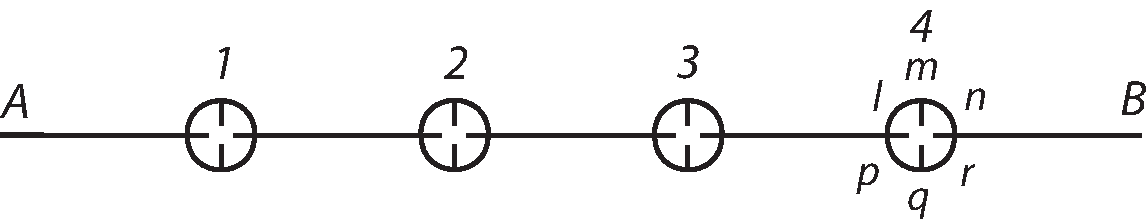
\includegraphics[width=0.64\textwidth]{gesamttex/edit_VIII,3/images/LH_37_01_016_d1.pdf}}%\\
  \vspace*{-0.5em}
  \centerline{\lbrack\textit{Fig.~1}\rbrack}
\newpage
\pstart
\noindent
retur\lbrack,\rbrack\
non eodem tempore restituetur\protect\index{Sachverzeichnis}{tempus restitutionis}
valde compressum ac parum compressum,\protect\index{Sachverzeichnis}{elaterium compressum}
nam extraneum aliquid praeterea agendum est magis in uno quam in altero.
Hinc jam aeris resistentia\protect\index{Sachverzeichnis}{resistentia aeris}
et ipsum pondus chordae\protect\index{Sachverzeichnis}{pondus chordae}
efficient ut non sit perfectus isochronismus.\protect\index{Sachverzeichnis}{isochronismus restitutionis}
\pend%
%\newpage
%
\count\Bfootins=1200
\count\Afootins=1200
\count\Cfootins=1200
\pstart%
Celeritas\edlabel{LH_37_01_016r_isochr-1}\protect\index{Sachverzeichnis}{celeritas restitutionis}
determinatur tum a nisu\protect\index{Sachverzeichnis}{nisus restitutionis}
seu potentia agente,\protect\index{Sachverzeichnis}{potentia agens}
tum a resistentia rei movendae.\protect\index{Sachverzeichnis}{resistentia rei movendae}
Sed si ab hac abstrahamus animum;\protect\index{Sachverzeichnis}{animus}
patet celeritates\protect\index{Sachverzeichnis}{celeritas restitutionis}
esse temporibus\protect\index{Sachverzeichnis}{tempus restitutionis}
reciproce proportionales,
ergo tempora reciproce proportionalia nisibus;
nisus autem sunt in composita ratione potentiarum
et turbationum,\protect\index{Sachverzeichnis}{turbatio}
et nisus\protect\index{Sachverzeichnis}{nisus restitutionis}
ejusdem potentiae\protect\index{Sachverzeichnis}{potentia agens}
in ratione turbationum.
Ergo tempora\protect\index{Sachverzeichnis}{tempus restitutionis}
in reciproca ratione turbationum,
sed cum turbationes\protect\index{Sachverzeichnis}{turbatio}
quovis momento\protect\index{Sachverzeichnis}{momentum temporis}
\edtext{immutentur, et}{%
\lemma{immutentur,}\Bfootnote{%
\textit{(1)}~imo
\textit{(2)}~et~\textit{L}}}
eo minor sit nisus\protect\index{Sachverzeichnis}{nisus restitutionis}
sequens quo praecedens major fuit,
hinc progressio per curvam exprimenda\protect\index{Sachverzeichnis}{progressio per curvam exprimenda}
erit,
\edtext{et
%
\lbrack16~v\textsuperscript{o}\rbrack\ %%%% Bl. 16v.
%
res}{%
\lemma{et}\Bfootnote{%
\hspace{-0,5mm}\lbrack16~v\textsuperscript{o}\rbrack\
\textbar~et \textit{streicht Hrsg.}~%
\textbar\ res~%
\textit{L}}}
eo redibit, ut ostendatur,
eandem temporum\protect\index{Sachverzeichnis}{tempus restitutionis} summam esse.
Moles gravium\protect\index{Sachverzeichnis}{moles gravium} nihil obstabit,
quominus eodem tempore ad centrum terrae\protect\index{Sachverzeichnis}{centrum terrae} perveniant,
quia ipsa eorum moles est causa turbationis.%
\edlabel{LH_37_01_016v_isochr-2}\protect\index{Sachverzeichnis}{causa turbationis}
%
Videndum an dimidia chorda\protect\index{Sachverzeichnis}{chorda dimidia}
iisdem servatis duplo celerius vibret.
Et sic videtur.
Nam si tantundem tendatur quantum integra,
erit duplo magis tensa\protect\index{Sachverzeichnis}{chorda tensa}
seu vim\protect\index{Sachverzeichnis}{vis tendens}
\edtext{passa\lbrack,\rbrack\
\edtext{}{%
{\xxref{LH_37_01_016v_utcunque-1}{LH_37_01_016v_utcunque-2}}%
{\lemma{utcunque \lbrack...\rbrack\ modo}\Cfootnote{%
Leibniz meint hier wohl nicht mehr die Spannkraft, sondern die Aus\-len\-kung der Saite (\textit{pulsatio}).%
% Beides lässt sich im Lateinischen als \textit{tensio} bezeichnen.
}}}%
\edlabel{LH_37_01_016v_utcunque-1}%
utcunque autem tendatur semper}{%
\lemma{passa}\Bfootnote{%
\textit{(1)}~. Ergo
\textit{(2)}~semper
\textit{(3)}~utcunque autem tendatur semper~\textit{L}}}
vibrat eodem modo.\edlabel{LH_37_01_016v_utcunque-2}
%
Videretur ergo corpus Elasticum\protect\index{Sachverzeichnis}{corpus elasticum}
omne quanto est minus,
\edtext{eo vibrare celerius.}{%
\lemma{eo}\Bfootnote{%
\textit{(1)}~fortius vibrare
\textit{(2)}~vibrare celerius.~\textit{L}}}
Etiam aerem ordinarium\protect\index{Sachverzeichnis}{aer ordinarius}
unius pedis cubici\protect\index{Sachverzeichnis}{pes cubicus}
fortius vibrare quam aerem duorum pedum cubicorum.
Quod rursus mirabile est.\edlabel{LH_37_01_016r_abschnitt_2-2}
\pend%
%
\pstart%
Sonus\edlabel{LH_37_01_016r_abschnitt_3-1}\protect\index{Sachverzeichnis}{sonus}
igitur pendet a partibus\protect\index{Sachverzeichnis}{pars aeris}
in quas aer vibratione\protect\index{Sachverzeichnis}{vibratio aeris}
quasi dissilit,
et quae et ipsae vibrant et vicinas excitant,
nam quo minores illae, hoc sonus
\edtext{acutior.\protect\index{Sachverzeichnis}{sonus acutus}
Modus quo}{%
\lemma{acutior.}\Bfootnote{%
\textit{(1)}~Cum ab vi
\textit{(2)}~Modus quo~\textit{L}}}
aer dissilit\lbrack,\rbrack\
hic esse videtur:
chorda\protect\index{Sachverzeichnis}{chorda vibrans}
\edtext{vibrans circumjacentem aerem\protect\index{Sachverzeichnis}{aer circumjacens}
impellendo comprimit, is\protect\index{Sachverzeichnis}{aer compressus}}{%
\lemma{vibrans}\Bfootnote{%
\textit{(1)}~imprimit aer
\textit{(2)}~circumjacentem aerem 
\textit{(a)}~premit et comprimit
\textit{(b)}~impellendo comprimit, 
\textit{(aa)}~itaque
\textit{(bb)}~is~\textit{L}}}
proprio nisu\protect\index{Sachverzeichnis}{nisus restitutionis}
se restituit et vibrat,
variae autem ob ejus liquiditatem\protect\index{Sachverzeichnis}{liquiditas}
in eo fiunt vibrationes,\protect\index{Sachverzeichnis}{vibratio aeris}
partium scilicet aliarum majorum aliarum minorum,
\edtext{sed partes mediae\protect\index{Sachverzeichnis}{pars aeris}}{%
\lemma{sed}\Bfootnote{%
\textit{(1)}~eae
\textit{(2)}~partes mediae%
~\textit{L}}}
quarum magnitudo talis est,
ut simul vibrent cum chorda,\protect\index{Sachverzeichnis}{chorda vibrans}
eae in vibratione perserverant,
reliquarum vibrationes destruuntur;\protect\index{Sachverzeichnis}{pars aeris}
et hae similiter vibrationem\protect\index{Sachverzeichnis}{vibratio aeris}
suam propagant in alias vicinas,\protect\index{Sachverzeichnis}{propagatio vibrationis}
et ita porro, usque ad aurem.\protect\index{Sachverzeichnis}{auris}
In aure
\edtext{autem potest fieri,
ut vel 
\edtext{}{%
{\xxref{LH_37_01_016v_tymp-1}{LH_37_01_016v_tymp-2}}%
{\lemma{tympanum \lbrack...\rbrack\ allapsi}\Cfootnote{%
Siehe zu dieser Auffassung der Funktion des Trommelfells etwa
H.~\textsc{Fabri}, \textit{Physica}, tract.~III, lib.~II, prop.~52 (Bd.~II, Lyon 1670, S.~152b\textendash153a)\cite{00044}.
Eine ähnliche Überlegung findet sich auch in \cite{00087}J.~\textsc{Rohault}, \textit{Traité de physique}, partie I, chap.~26, §~48 (2. Ausgabe, Paris 1672, Bd.~I, S.~290).}}}%
\edlabel{LH_37_01_016v_tymp-1}tympanum\protect\index{Sachverzeichnis}{tympanum} ipsum}{%
\lemma{autem}\Bfootnote{%
\textit{(1)}~possunt in ipso tympan
\textit{(2)}~potest fieri, ut vel tympanum ipsum~\textit{L}}}
varie intendamus pro ratione soni allapsi,%
\edlabel{LH_37_01_016v_tymp-2}\protect\index{Sachverzeichnis}{sonus allapsus}
%
vel ut tympanum\protect\index{Sachverzeichnis}{tympanum}
ex diversae tensionis\protect\index{Sachverzeichnis}{tensio} constet partibus,
quarum aliae ab hoc, aliae ab alio sono\protect\index{Sachverzeichnis}{sonus allapsus}
\edtext{pulsentur ut}{%
\lemma{pulsentur}\Bfootnote{%
\textit{(1)}~. Et hoc modo
\textit{(2)}~ut~\textit{L}}}
chordae chordis unisonis\protect\index{Sachverzeichnis}{chorda unisona}
pulsatis\protect\index{Sachverzeichnis}{chorda pulsata}
consonant\protect\index{Sachverzeichnis}{chorda consonans}
etsi non nisi ab aere pulsentur.\edlabel{LH_37_01_016r_abschnitt_3-2}
\pend%
%\newpage%
\pstart%
Videndum\edlabel{LH_37_01_016r_abschnitt_4-1} an verum sit, et ex
\edtext{his demonstrari queat,}{%
\lemma{his}\Bfootnote{%
\textit{(1)}~demonstretur
\textit{(2)}~demonstrari queat,~\textit{L}}}
quod omnis sonus\protect\index{Sachverzeichnis}{sonus} feratur\edlabel{LH_37_01_016v_Schallgeschwindigkeit-1}
\edtext{uniformi velocitate,%
\protect\index{Sachverzeichnis}{velocitas uniformis}\protect\index{Sachverzeichnis}{velocitas soni}
seu ut celeritas\protect\index{Sachverzeichnis}{celeritas soni}
sit in ratione distantiarum,\protect\index{Sachverzeichnis}{distantia}\edlabel{LH_37_01_016v_Schallgeschwindigkeit-2}}{%
\lemma{uniformi \lbrack...\rbrack\ distantiarum}\Cfootnote{%
Leibniz äußert sich hier widersprüchlich.
Siehe für eine angemessene Darstellung der gleichförmigen Geschwindigkeit der Schallausbreitung vielmehr
G.\,W. \textsc{Leibniz}, Brief an G.\,C. Schelhammer vom Februar/März 1681 (\textit{LSB} III,~3 N.~182, S.~359.14\textendash360.1)
sowie hier unten, N.~12\textsubscript{1}, S.~\refpassage{LH_37_01_019r_gleichscnell-1}{LH_37_01_019r_gleichscnell-2}.}}
et hoc verum puto,
prorsus ac si elateria\protect\index{Sachverzeichnis}{elaterium} similia in
\edtext{longam seriem disposita\protect\index{Sachverzeichnis}{series elateriorum}
sese ordine\protect\index{Sachverzeichnis}{ordo} liberent}{%
\lemma{longam}\Bfootnote{%
\textit{(1)}~distantiam se
\textit{(2)}~seriem disposita
\textit{(a)}~se mutuo liberent
\textit{(b)}~sese ordine liberent%
~\textit{L}}}
%
\lbrack\textit{danach gestrichen und abbrechend:}\rbrack\
\footnotesize{%
vel pulsent.
Si
\edtext{chordae\protect\index{Sachverzeichnis}{chorda parallela} parallelae}{%
\lemma{chordae}\Bfootnote{%
\textit{(1)}~vi
\textit{(2)}~parallelae%
~\textit{L}}}
%
eodem modo tensae\protect\index{Sachverzeichnis}{chorda tensa} sint numero quotcunque,
et una pulsata\protect\index{Sachverzeichnis}{chorda pulsata} aliam
\edtext{pulset; aliae consonant;}{%
\lemma{pulset;}\Bfootnote{%
\textit{(1)}~$\langle$nec$\rangle$
\textit{(2)}~pulsando
\textit{(a)}~aliquid
\textit{(b)}~aliquid
\textit{(3)}~manifestum est
\textit{(4)}~aliae consonant;%
~\textit{L}}}}%
%
% \lbrack\textit{Text bricht ab.}\rbrack%
\edlabel{LH_37_01_016r_abschnitt_4-2}
\normalsize%
\pend%
%
% \newpage%
\vspace*{3.0em}%
%
\pstart%
\setline{1}
  \centerline{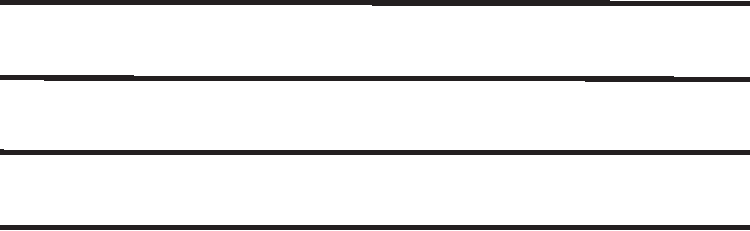
\includegraphics[width=0.35\textwidth]{gesamttex/edit_VIII,3/images/LH_37_01_016_d2.pdf}}%\\
  \vspace*{0.5em}
  \centerline{\lbrack\textit{Fig. 2}\rbrack}%
\edtext{}{\lemma{\hspace*{1,6mm}\lbrack\textit{Fig.~2}\rbrack}\killnumber\Cfootnote{Ungestrichene Zeichnung zu den gestrichenen Zeilen am Ende des Textes.
Sie ähnelt den Diagrammen \lbrack\textit{Fig.~1}\rbrack\ in N.~12\textsubscript{1}, S.~\pageref{LH_37_01_018v_Fig.1}, und \lbrack\textit{Fig.~2}\rbrack\ in N.~12\textsubscript{3}, % S.~\pageref{LH_37_01_001-002_d2}, und ??X\textsubscript{4}, 
S.~\pageref{LH_37_01_005r_Fig.2}.}}%
\pend%
\count\Bfootins=1200
\count\Afootins=1200
\count\Cfootins=1200
%
% ENDE DES STÜCKES auf Bl. 16v.